\chapter{Background}\label{chp.background}
In this Chapter, the book which this work based on, ``The Lonely Crowd'' and its author David Riesman are introduced in the Section~\ref{chp.background.david}. As the main part of the book, the definition and characteristics of the concept ``social character'' are first introduced, based on the works from Erich Fromm. Afterwards, three social characters, identified by David Riesman are introduced in Section~\ref{chp.background.characters}. 

\section{David Riesman and His Work}\label{chp.background.david}

David Riesman was a sociologist, educator, and best-selling commentator on American society. Born to a wealthy German Jewish family in 1909, he graduated from Harvard College with a degree in biochemistry in 1931, then earned his law degree from Harvard Law School. Afterwards, he taught at the University of Buffalo Law School and at the University of Chicago. In the late 1940s, he took a leave from Chicago to focus on a project at Yale, which sponsored the work that led to ``The Lonely Crowd''. In 1958, he left Chicago for a
position as University Professor at Harvard, where he
remained for the rest of his teaching career and passed by in 2002.

As the most famous work of David Riesman, the book ``The Lonely Crowd'', first published in 1950 as a sociological analysis of American life, became a surprising bestseller and is considered to be the most influential book of the twentieth century~\citep{riesman1979making}. According to~\citeauthor{horowitz2010david}, It is also the nation’s most influential and widely read mid-century work of social and cultural criticism and catapulted its author to the cover of Time magazine in 1954, making David Riesman the first social scientist so honored~\citep{horowitz2010david}. As historian
Rupert Wilkinson suggests, ```The Lonely Crowd' heralded later findings to a degree that is seldom appreciated. Narcissism
and `diffuse anxiety'; the shifting of authority from `dos and don'ts' to manipulation and enticement; the flooding of attitudes by media messages; the channeling of achievement drives into competition for the approval of others; and the splintering of society into myriad interest groups--all these tendencies of modern American life that so worried commentators in the 1970s and 80s were spotted by Riesman et al.''~\citep{wilkinson1988pursuit}. In the book, following topics are mainly introduced and discussed.
\begin{itemize}
\item[1] Three social characters and their different characteristics.%which will be shortly introduced in Section~\ref{chp.background.characters}.  
\item[2] The way different social characters prevail in the work, in leisure, in politics and in education. %In this work, the influence of the other-directed type is introduced in Section~\ref{chp.Criticism.Book}.  
\item[3] The transition of the social characters, namely, a gradual replacement by a social character of a completely different kind.% which is introduced in ~\ref{chp.background.characters} and~\ref{chp.Criticism.Comparison}.
\item[4] Why and how this replacement took place and how it affects some major areas of life.
\end{itemize}
 
\section{Social characters and Transitions}\label{chp.background.characters}  

\textbf{Erich Fromm.}
The social character is the central basic concept of the analytic social psychology of Erich Fromm, who was a German psychoanalyst, sociologist and former member of the Institute for
Social Research in Frankfurt. The concept integrates Marx's theory concerning how the mode of production determines ideology with Freud's concept of character~\citep{fromm1941escape}.

While individual character describes the richness of the character structure of an individual, the social character describes the common of the emotional attitudes and psychological reactions to people in a social class or society. In particular, the concept describes the formation of the shared character structure of the people of a society or a social class according to their way of life, the socially typical expectations and functional requirements regarding socially adaptive behavior. The social character is necessary to be acquired and obeyed by the members of a society, enabling their members to do what they need to do in order to prosper and enabling a society to function adequately~\citep{fromm1941escape, fromm1994escape}.

Although everyone develops character traits and character orientations that distinguish them from people who live in other cultures, people in every culture with the same mode of production share basic elements of the social character~\citep{fromm1970social}, making it possible to generate the social character in one culture to other cultures. For example, three social characters based on the American society in the book ``The Lonely Crowd'' are not limited in the United States but also have a certain reference value to other cultures, which could explain, in some degree, why the book became the best-seller all over the world.

\textbf{David Riesman.}~As a patient of the therapist Erich Fromm in the early 1940s, David Riesman was influenced intellectually and personally, due to an unconventional psychoanalysis, which resembles a teacher/student rather than a psychoanalyst/patient relationship, resulting in his interest in sociology and further extension of the concept ``social character'' in his work ``the Lonely Crowd''. In the book, three types of social characters: the tradition-directed, the inner-directed, and the other-directed type are identified and analyzed as well as the transitions between them.

\begin{figure}{t!}
  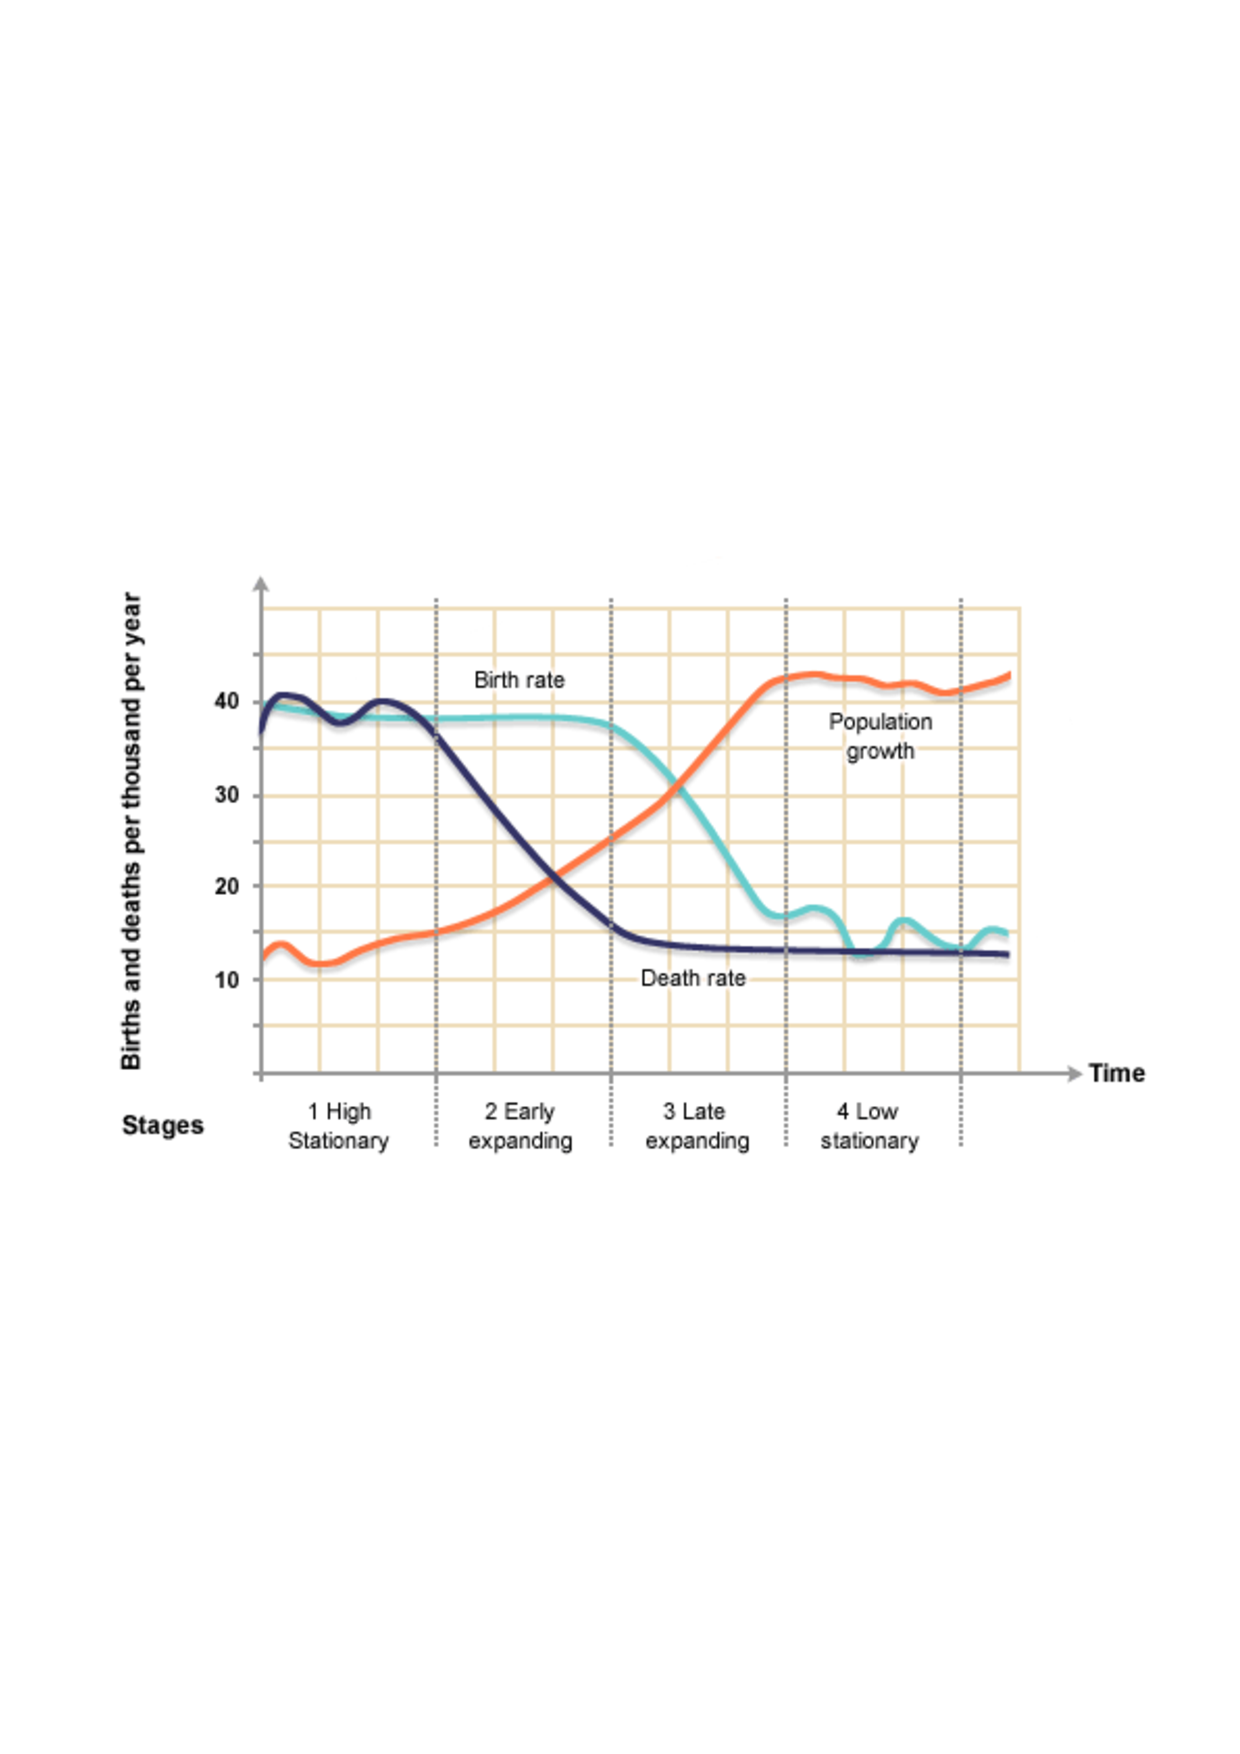
\includegraphics[width=\linewidth]{population_changes.pdf}
  \caption{The changes in the birth and death rates as well as the population growth during the transitions}
  \label{background.fig.population}
\end{figure}


\textbf{The tradition-directed type} dominates in the primitive societies, where both birth rate and death rate were high (refers to the first stage in Figure~\ref{background.fig.population}). Its members are with a low level of individualism and strong ties to primary groups, obeying rules established a long time in the past. This kind of social character has, according to Riesman, disappeared in the modern American
society, except in pockets of black, French Canadian, Southern, rural and immigrant cultures. 

Due to the drop of death rate in industrial economies (refers to the second stage in Figure~\ref{background.fig.population}), as well as industrialization, urbanization and modern technology, there was an intensive expansion of goods and people. As a result, many novel situations were presented, where a strict code could not encompass in advance like in the tradition-directed society and the control of the primary group in a tradition directed society was loosened. Therefore,~\textbf{the inner-directed type} became dominant, offering a wide choice but stable at the same time, whose members discovered the potential within themselves to live and act not according to the established norms but based on what they discovered using their own inner gyroscope that were essentially ``implanted'' by elders. Compared to the other-directed type, the inner-directed type of social character is focused on producing than consuming, whose members conform their outward behaviors, like dressing, to match societal norms, while the opinions of others have little sway on their inner lives, for example, the goal of pursuing money and rights. In other words, They would rather be esteemed than be loved.

In the mid twenties century, as the birth rate begins to follow the death rate downward (refers to the third and fourth stage in Figure~\ref{background.fig.population}), societies move toward the epoch of incipient decline of population and of service, trade and communications-driven economy. Fewer and fewer people work, hours are short, people may have material abundance and leisure besides, who are mixed more widely and thereafter becoming more sensitive to each other, since material environment is no longer a problem. Therefore, the social character was shifting from a 19th-century inner-directed type to a mid-20th-century~\textbf{other-directed type}, dominated by a concern for ``niceness'' instead of achievement, leisure instead of competition and ``consumerism'' instead of production. However, due to the lack of the cultural expectations for how to live, the other-directed people look to their peers and the media for guidance, making them very sensitive to the preferences and expectations of others using a ``radar''. Compared to inner-directed people, they would rather be loved than esteemed. In particular, modern parents and teachers are anxiety ridden as their authority over children and students has been undermined by the media, youth culture and a rapid social change that creates a situation where the ``other-directed child is often more knowing than his parents''. 


			

			
		

